\chapter{Compressive UWB Positioning}\label{C:compressive_uwb_positioning}
\indent \indent In this chapter, we first present an overview of UWB communication, and then focus on on our related work in Impulse-radio ultra-wideband (UWB) positioning system. The proposed work shows the potential advantages if we implement CS projection in the transmitter of the UWB positioning system according to the experiment result. Besides, Our proposed compressive UWB positioning presents a novel view of energy trade-off design, which is implemented by a low-rate random-projection at transmitters and low rate ADCs at receivers. It is clear that this design significantly reduce the peak frequency in the system with acceptable rate increase in receivers' ADC sampling rate.   

\section{Introduction}
\indent \indent Ultra-wide band (UWB) communication is widely used in wireless communication and associated with features as extreme wide transmission bandwidth, low-power consumption, shared spectrum resources in wide ranges etc \cite{paredes2007ultra}. Among all applicable areas, UWB based accurate positioning and tracking in short range communication become popular since it provides resilient to multipath fading in hostile environment and outstanding robustness even in low signal-to-noise (SNR) situations \cite{cassioli2002ultra}. In addition, the requirements of high data rate and limitations of battery supply lead the impulse-radio ultra-wide band (IR-UWB) to become a suitable communication technique in short range high data rate communication. As a result, applications based short-distance wireless sensor networks (WSNs) where large numbers of portable instrument, are widely deployed such as indoor positioning, surveillance, home automation, etc. 

However, high data rate transmission puts huge pressure on signal detection at ADCs at receivers, which indicates the sampling rate becomes a main bottleneck to the IR-UWB system. This paper focuses on the IR-UWB indoor positioning, aims at solving the bottleneck of sampling rate by using a recent novel technique termed compressed sensing (CS), aforementioned in Chapter \ref{C:compressed_sensing}. Compressed sensing is a novel paradigm which applies randomly sampling and sparse reconstruction, which enables a possible reconstruction strategy for sparse signals from a relatively small group of random measurements. It indicates that CS based IR-UWB systems can possibly detect high frequency sparse signals under a sub-Nyquist sampling rates that far below the Nyquist rate (twice the IR-UWB bandwidth). This result is advantageous which releases the bottleneck of the large bandwidth constraints on ADC at UWB receivers, and consequently reduces storage limits and improves energy efficiency in IR-UWB positioning systems.

Recently some researches manage to embed CS reconstruction algorithms, e.g. revised orthogonal matching pursuit, at UWB receivers. These algorithms successfully improve the SNR of the received signal before they are sent to the stages of time of arrival (TOA) based positioning algorithm. Consequently, this method increases the performance of entire positioning accuracy \cite{banitalebi2014compressive}. For hardware implementation of the new CS based UWB receivers, most of them apply the hardware structure termed the random demodulator (RD) \cite{kirolos2006analog}, and consequently this new CS-UWB receiver successfully reduces the sampling rate significantly compared to the Nyquist rate \cite{yang2011compressive}.

On the other hand, some researches embed the CS technique mainly at UWB transmitters. They develop a waveform-based precoding transmitter, in order to fulfil a random projection of the UWB generated pulses \cite{zhang2009compressed}. Followed by sub-Nyquist sampling ADCs at receivers, the sampled signals are sent to TOA based algorithm for calculating the location of the UWB transmitter. Simulation results show that the new CS-UWB transmitter manage to significantly decrease the sampling rate of receivers successfully improves accuracy of traditional UWB positioning system. 

However, both CS-UWB receivers and CS-UWB transmitters suffer from high-data rate random mixing operation, where PN sequence at mixers is required to reach the extremely high Nyquist rate ( e.g. beyond 10 GHz). This requirement generates heavy burden on bandwidth of hardware mixers and additionally increases a high frequency noise. To solve this problem, this paper propose an advanced low-rate CS-UWB positioning system: For the CS-UWB transmitter, it implements a relatively low-rate random projection matrix to slow down the mixing rate. For CS-UWB receivers, they sacrifices a small degree of compression ratio to keep equivalent performance as those positioning system using traditional CS-UWB transmitters. As a result, the trade-off between the random mixing rate and the sub-Nyquist sampling rate makes our system to become a more energy balanced, and consequently gains a better performance in entire power consumption and energy efficiency.  

\section{Model of Traditional UWB Positioning}
\indent \indent Extremely wide transmission bandwidths of the IR-UWB offers outstanding multipath resolutions for accurate positioning in indoor environment. Consider a typical UWB indoor communication model where distributed UWB receivers (base stations) are placed in an area to detect the location of a moving UWB transmitter (tag). The transmitter periodically broadcasts Gaussian shaped pulse $p(t)$ through an indoor multipath channel, and receivers detect signals for time of arrival (TOA) based positioning calculation. The received signals can be described as (\ref{eq_recv}):
\begin{equation}
\label{eq_recv}
r(t) = p(t) * h(t) + n(t) = \sum_{l=1}^{L} a_l p(t-\tau_l) + n(t) 
\end{equation}
where $p(t)$ is the transmitted Gaussian pulse, $n(t)$ stands for zero-mean additive white Gaussian noise (AWGN), and $h(t)$ refers to the standard UWB channel model denoted by IEEE 802.15.4a (\ref{eq_chan}):
\begin{equation}
\label{eq_chan}
h(t) = \sum_{l=1}^{L} a_l \delta(t-\tau_l)
\end{equation}
Here $a_l$ and $\tau_l$ are the gain and delay corresponding to the $i$-th path in the channel model. The $L$ defines the total number of propagation paths, and $\delta(t)$ is the Dirac delta function. Based on the fact that geometrical difference yields different time of arrivals, the received signals at the different receivers are collected for TOA based algorithm. At last accurate position of the transmitter is calculated based on TOA \cite{d2010toa}. In addition, since both transmitted pulses and components of multipath channel can be regarded as approximately sparse, the received IR-UWB signals becomes sparse, and consequently the CS framework is applicable for UWB positioning \cite{yang2011compressive}. 

\section{Compressive UWB Positioning}
\indent \indent This section first discusses popular CS based architectures for UWB positioning. Next, a new structure of CS-UWB positioning will be introduced as the main contribution of this paper.    

\subsection{Compressive Receivers}
\begin{figure}[!t]
\centering
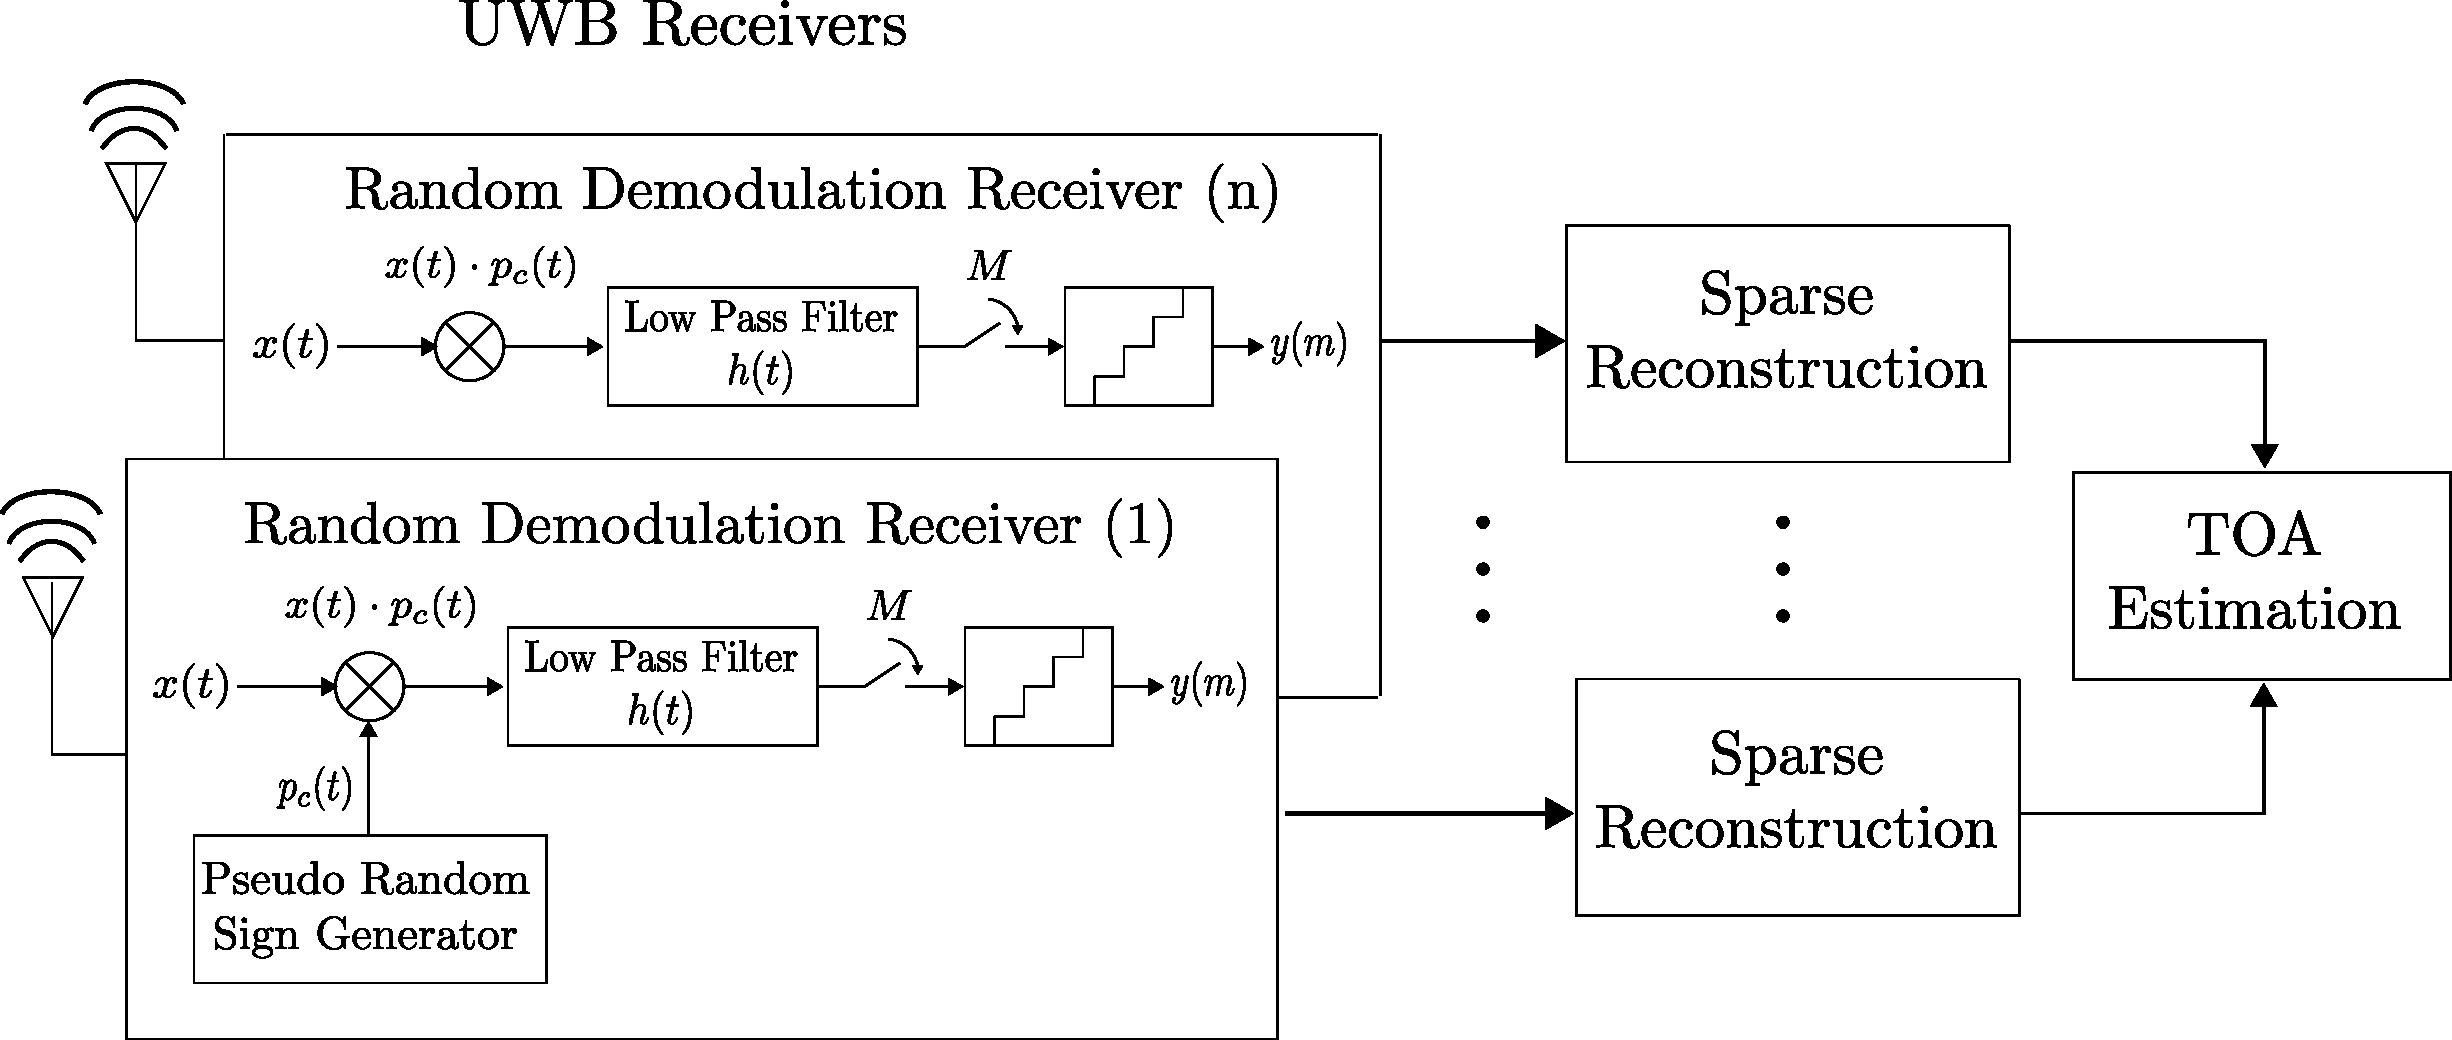
\includegraphics[width=0.5\columnwidth]{cs-uwb-design1.pdf}
\DeclareGraphicsExtensions.
\caption{Block diagram of compressive receiver implemented by random demodulator (RD). The components of RD includes a pseudo-random sign generator (PRSG), a low-pass filter (LPF), and a sub-Nyquist ADC}
\label{cs-uwb-design1}
\end{figure}

Typical recent researches embed the CS reconstruction algorithm at UWB receivers to improve the SNR of the received signal. As a result, it not only increases the performance of the positioning accuracy \cite{banitalebi2014compressive}, but also reduces the sampling rate to a relatively low level compared to the Nyquist rate. Among these compressive receivers, most of them develop the random demodulator (RD) \cite{kirolos2006analog} as the main structure of CS based UWB receivers \cite{yang2011compressive}. 

In this system, each compressive receiver realises the RD architecture that composed of a pseudo-random sign generator (PRSG), a low pass filter (LPF), and a sub-Nyquist rate analog-to-digital converter (ADC), shown in Fig.\ref{cs-uwb-design1}. 

Then the transmitted UWB signals are collected by group of low-rate distributed ADCs only using a minimal sampling rate of $1.7K(log(N/K))$ \cite{kirolos2006analog}, where $N$ stands for Nyquist rate and $K$ is the sparsity in transmitted UWB signals. Results in \cite{yang2013compressive} demonstrates that the new system successfully improves positioning accuracy. 

\subsection{Compressive Transmitters}
\indent \indent On the other hand, some researches embed the CS technique at the UWB transmitter and regarded it as a better solution than compressive receivers in terms of  system hardware power efficiency. The new architecture contains a random tap FIR at the transmitter, which accomplishes the CS random projection before UWB signals are transmitted \cite{zhang2009compressed}. Followed by distributed sub-Nyquist rate ADCs, the down-sampled signals are collected for TOA based algorithm. Simulation result \cite{zhang2009compressed} shows that the new compressive transmitter is suitable for detecting the indoor channel model with higher accuracy than traditional TOA based method. This architecture is also suitable for indoor positioning because the transmitted signal pulse and channel model keep the same. Besides, it meanwhile saves more energy cost since it contains less hardware mixers than compressive receiver based UWB system. However, the complexity of implementation a high data rate random tap FIR filters brings additional cost and becomes a main difficulty in applications.

\section{Energy Aware Random Mixing Transmitters}
\begin{figure*}[!t]
\centering
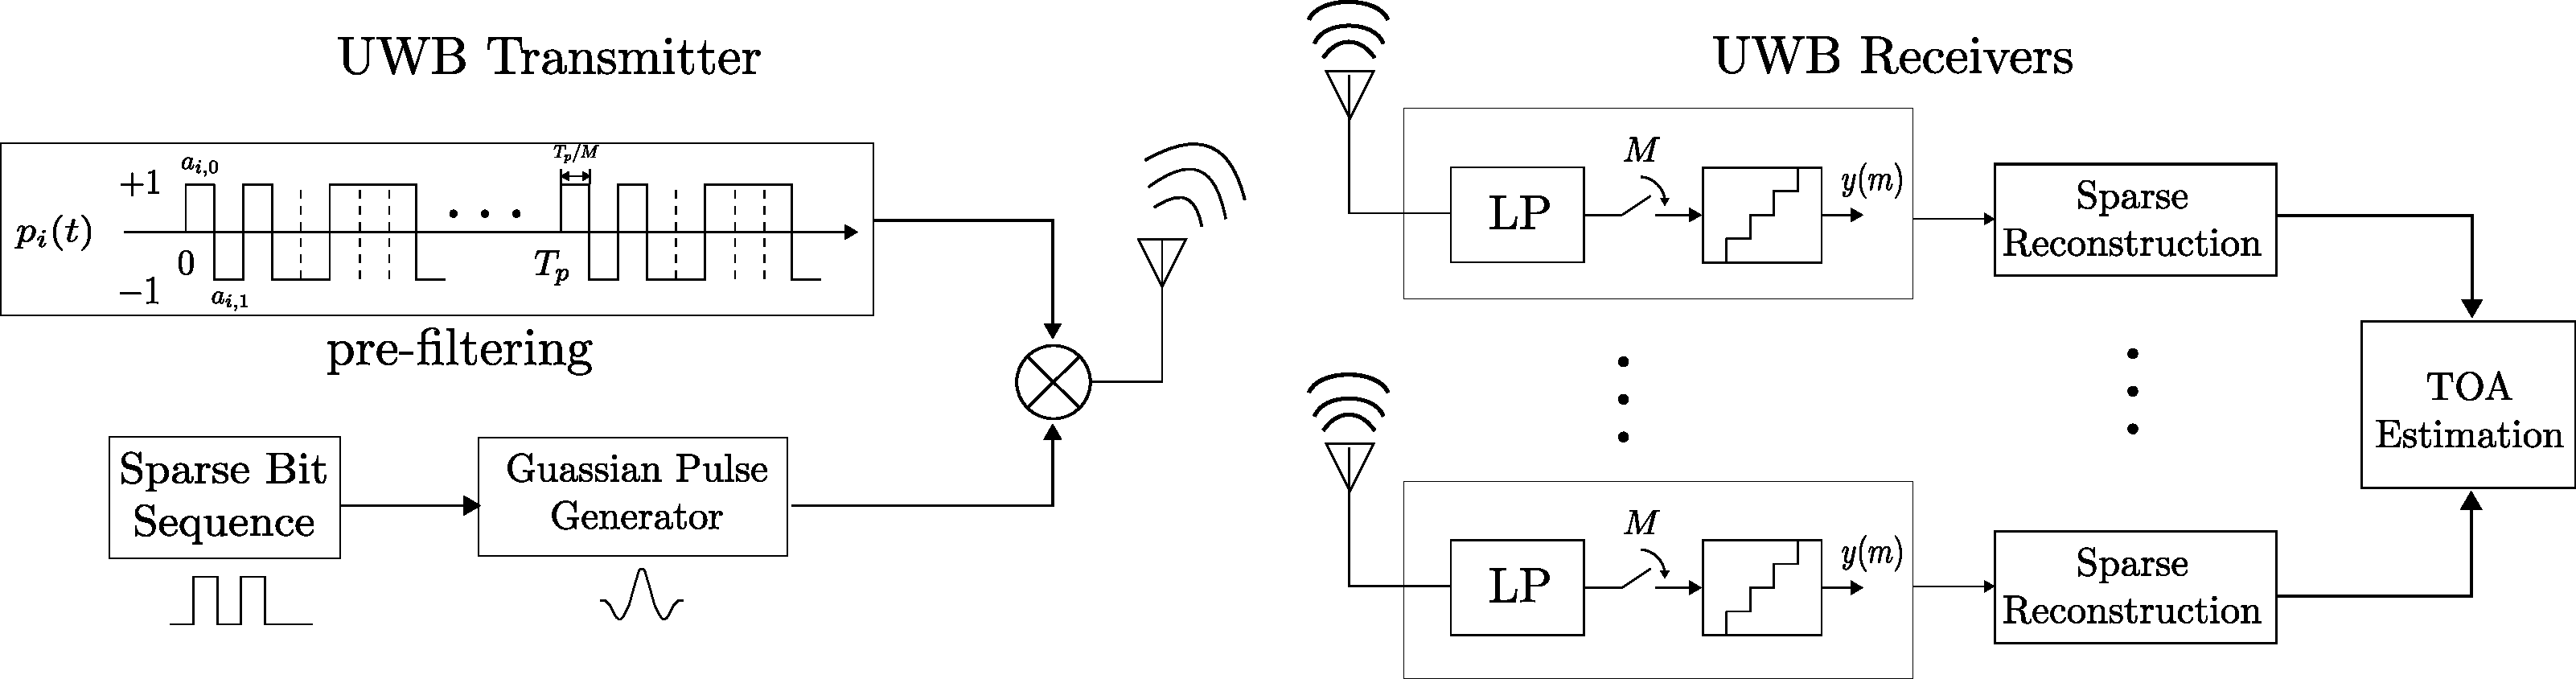
\includegraphics[width=0.85\columnwidth]{cs-uwb-design2.pdf}
\DeclareGraphicsExtensions.
\caption{Block diagram of low-rate compressive random mixing UWB positioning system.}
\label{cs-uwb-design2}
\end{figure*}

As mentioned, both compressive receivers and compressive transmitters suffer from high-data rate random projection operation, where the alternative rate of pseudo-random sequence is required (often equal or above 5 GHz in such cases). This requirement generates a heavy burden on bandwidth of hardware mixers and high frequency noise. 

In order to solve this problem but meanwhile preserve the energy efficient feature in compressive transmitters, this paper propose an low-rate compressive random mixing (CRM) UWB positioning system shown in Fig.\ref{cs-uwb-design2}: At the transmitter side, the new system provides a relatively low-rate pseudo-random sequence to mix the generated Gaussian pulses. At the receivers side, it sacrifices the compression ratio (or sampling rate) to catch up with the equivalent performance as that in the compressive receivers based UWB system. As a result, the trade-off between the random projection rate and the sub-Nyquist sampling rate offers a more energetic balanced system, where no hardware devices suffers from the limitation brought from the high data rate sequence. In addition, the positioning accuracy is successfully improved compared to the original UWB system. 

\paragraph{System Model}
Based on the IR-UWB indoor positioning system model in (\ref{eq_recv}), the new structure of our system can be regarded as shown in Fig.\ref{cs-uwb-design2}. At the transmitter, the a pseudo-random sequence (PRS) whose variables are chosen from ${-1,+1}$ are generated using a relatively low sub-Nyquist alternative rate. When a UWB pulse generated, first it will be randomly mixed by the pseudo-random sequence, and then broadcasted to indoor environment from the transmitter. Afterwards, receivers directly down-sample the signals at a relatively low rate. Finally, after processing the sparse reconstruction (i.e OMP or BP), the original TOA based algorithm can work for indoor positioning. In addition, these steps at receivers can be executed pipelined as \cite{yang2011compressive}. Hence, based on the workflow of the new architecture, the math model of this system can be represented as following matrix form (\ref{eq_sys_m}):
\begin{equation}
\label{eq_sys_m}
y = D * H * P * x
\end{equation}
where $y$ are discrete sampled observations from low rate ADCs at receivers, and $x$ is the generated UWB Gaussian pulses at traditional transmitters. Here $H$ is the correspondingly Toeplitz matrix which presents the signal convolution using IEEE 802.15.4a model in (\ref{eq_chan}), and $F$ stands for the random projection step, which is a diagnose matrix whose variables are randomly chosen from $\{-1,+1\}$ but alternatives at a sub-Nyquist low rate. The $D$ represents the downsampling behaviour. It is a $m\times N$ matrix ($m << N$) with 0-1 entries , and each of its rows contains a block of $\frac{m}/{N}$ contiguous ones, which has been used for simulation in \cite{tropp2010beyond}. Then $\hat x$ can be reconstructed from various sparse reconstruction algorithm such as BP, OMP and CoSaMP. At last, the recovered signal $\hat x$ is applied for TOA based positioning estimation.

\section{Simulation Results}
\indent \indent This experiment uses Matlab to evaluate the performance of the proposed system. In the simulation, the UWB waveform is a periodic simple pulse which is shaped by the second derivative Gaussian wave with a pulse duration of 1ns. The bandwidth of this signal is 8GHz. The UWB channel model is based on the IEEE 802.15.4a CM1 model for line of sight (LOS) indoor environment, and zero-mean additive white Gaussian noise (AWGN) is added to generate an average SNR of 10dB. The simulation results cover random points in an area of 10m $\times$ 10m $\times$ 10m space.

CS Basis pursuit denoising (BPDN) algorithm is used at the receiver to perform the reconstruction process. Figure 4 shows the results of the reconstruction successful rate against the receiver’s sampling rates. Existing RD based system achieves $100\%$ successful reconstruction starting at 200MHz sampling rate, but requires 10GHz PN sequence at each receiver. Our proposed system use much lower rate PN sequence (1GHz or 500MHz) at the transmitter and achieve $100\%$ successful reconstruction at 350MHz and 500MHz sampling rate. Hence, accuracy of the lower rate PN sequence system can be improved by using higher sampling rate at the receiver. Therefore, the simulation result shows that the proposed system can apply trade-off among random projection rate, sub-Nyquist sampling rate and reconstruction rate. This design significantly reduce the peak frequency (Nyquist rate in mixing waveform or receiving end) in the system with acceptable rate increase in receivers' ADC sampling rate. 

Table I compares the accuracy of the two CS based systems against conventional UWB based system which uses hypothetical 10GHz Nyquist sampling rate. Both CS based systems produces much lower errors then the conventional UWB based system, while the proposed RP system has similar performance as the RD based system. 

\begin{figure}[!t]
\centering
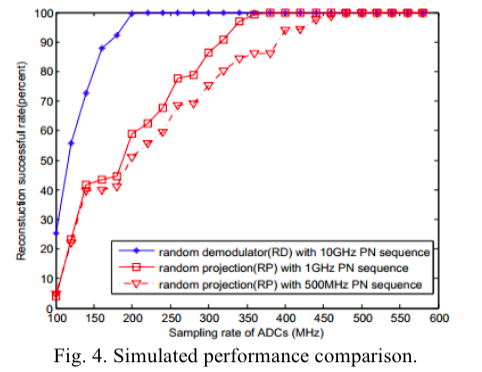
\includegraphics[width=0.5\columnwidth]{figs/res-pub.png}
\DeclareGraphicsExtensions.
%\caption{CS based TOA estimation average error under different compression ratio based on the IEEE 802.15.4a CM1 model for line of sight (LOS) indoor environment}
\label{res-pub}
\end{figure}
\begin{figure}[!t]
\centering
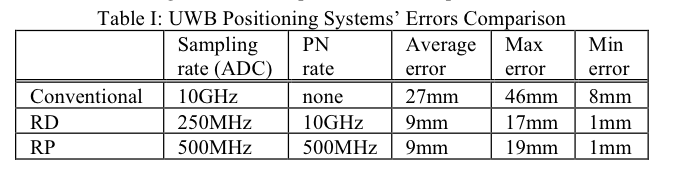
\includegraphics[width=0.75\columnwidth]{figs/res-pub-table.png}
\DeclareGraphicsExtensions.
%\caption{CS based TOA estimation average error under different compression ratio based on the IEEE 802.15.4a CM1 model for line of sight (LOS) indoor environment}
\label{res-temp}
\end{figure}

\section{Conclusion}\label{sct:cs_uwb_conclusion}
\indent \indent The compressed sensing is proven effective to improve the accuracy of IR-UWB positioning. However, most of papers do not concern the design complexity and energy cost in their implementations, for instance, the random mixing waveform is of extremely high frequency (in GHz). Our proposed compressive UWB positioning present a novel view of energy trade-off design, which is implemented by a low-rate random-projection at transmitters and low rate ADCs at receivers. This design significantly reduce the peak frequency (Nyquist rate in mixing waveform or receiving end) in the system with acceptable rate increase in receivers' ADC sampling rate. 

In this paper, following the architecture of waveform-based pre-coding at the transmitter\cite{zhang2009compressed}, we proposed a new compressive random mixing transmitters for UWB positioning. The main purpose of this system is to slow down the high rate mixing operation when building CS framework at transmitters. Simulation results demonstrate that our proposed CS-based UWB positioning scheme successfully decreases the high rate mixing operation by sacrificing a slight compression ratio ($<$ 10\%) or small increase on average error ($<$ 1mm). The new CS-UWB TOA positioning system can achieve a much higher positioning accuracy than the traditional system in mm level. Future research will focus on how to reduce the reconstruction running time so that the real-time performance can be enhanced. This aim relates to the compressive signal processing that will be mentioned in the next chapter.

%----------------------------------------------
%\section{Challenges in Ultra-Wideband System}

%Impulse-radio ultra wideband (UWB) technology has attracted widely usage in communication and positioning application, because of its advantages of extreme wide transmission bandwidth, fine time resolution, low-power consumption, low fading margin in dense multipath environment. There are two primary challenges exist, which are (1) how to gather energy over the rich multipath components, and (2) how to sample extremely high rate signals\cite{zhang2009compressed}. 

%%Additionally, in 2002, the FCC issued a first report and order allowing the unlicensed use of UWB devices, overlaid with existing devices, subject to a power spectral mask in a 7.5 GHz swath of spectrum. This has generated wide interest in potential UWB applications, and led to a rapid increase in the number of companies and governmental agencies working in UWB.

%%Many investigated applications for UWB are designed to operate in indoor environments. Indoor UWB systems must contend with dense multipath channels, which are characterised by tens or even hundreds of resolvable multipath components, and delay spreads typically orders of magnitude larger than the UWB pulse duration. Additionally, due to stringent FCC regulations, UWB systems are required to operate at a very low power emission level. These facts have led to several challenges pertaining to UWB transceiver design. Specifically, there are open challenges to be met in the areas of (a) UWB signal detection, (b) synchronisation, and (c) interference mitigation.

%%(1) Signal detection: Recent research has mainly concentrated on the Rake receiver and variants of the transmitted reference receiver as candidates for UWB detectors in dense multipath. However, both receivers have severe performance limitations. Specifically, the energy capture of the Rake receiver is relatively low for a moderate number of fingers, making its implementation impractical for UWB systems. Transmitted reference receivers suffer from a “noise-cross-noise” term, caused by the use of a noisy signal as a correlation or matched filter template. Consequently, a prohibitively large number of pilot symbols are required to overcome this limitation.

%Time reversal [5] provides a promising solution to the first problem [6]. In particular, the concept of time reversal has recently demonstrated in a real-time hardware test-bed [7], [8]. At the heart of time reversal, the channel itself is exploited as a part of the transceiver. This idea makes sense since the channel is time-invariant and reciprocal [9]. In principle, most of the processing at the receiver can be moved to the transmitter where energy consumption and computation are sufficient for many advanced algorithms. This framework is called waveform-oriented pre-coding.

%For instance, ultra-wide band (UWB) positioning always suffers from extremely high-rate signal detection. The compressive sensing (CS), which is considered as the optimal solution of acquisition and reconstruction for sparse signals, provides an alternative solution by implementing random projection at transmitters or receivers. However, these CS based UWB positioning systems still cannot avoid high-rate mixing operation when generating the PN sequence during random projection. 

%In this paper, we propose a new CS based UWB positioning system to solve this problem, which implements a relatively low-rate random pre-mixing at the transmitter and correspondingly sub-Nyquist rate sampling at receivers. As a result, the new system successfully eliminates the extremely high Nyquist rate in the system by sacrifices a small degree of compression ratio. Simulation results demonstrate the new system maintains outstanding performance in terms of positioning accuracy. 


%----UWB short introduction----

%\indent \indent Ultra-wide band (UWB) communication is widely used in wireless communication and associated with features as extreme wide transmission bandwidth, low-power consumption, shared spectrum resources in wide ranges etc. Among all applicable areas, UWB based accurate positioning and tracking in short range communication become popular since it provide resilient to multipath fading in hostile environment and outstanding robustness even in low signal-to-noise (SNR) situations \cite{cassioli2002ultra}. In addition, the requirements of high data rate and limitations of battery supply lead the impulse-radio ultra-wide band (IR-UWB) to become a suitable communication technique in short range high data rate communication. 

%However, along with the ultra high frequency transmission in IR-UWB communication, the receiving-end are suffering high sampling rate difficulty on its ADCs. Although many filter-bank based downsampling technologies are used to convert the high frequency into low frequency of original signal, complexity of multiple analog filters increase the design cost for hardware implementations.   

%Recently the CS framework is introduced to solve this problem for UWB, which provide a more convenient way to reduce the sampling rate at receivers. Comparing to traditional methods, the CS-based UWB omits the multiple analog filters and thus reduce the design complexity and cost. Simulation results demonstrate that the CS-UWB positioning can achieve high accuracy performance and providing energy-efficient design. 

%Our proposed work for UWB positioning system follows this idea, and additionally, we consider a further energy optimisation from aspect of architecture. While the formal CS-UWB uses Nyquist rate chipping sequence (or PN sequence) to fulfil random sampling behaviour for CS framework, however, this procedure forces Nyquist sequence and thus the high frequency does NOT omitted although sampling rate has been reduced. Our design aims at this problem, analyses a tradeoff between the rate of PN sequence and the sampling rate, and finally eliminates the Nyquist rate in entire system.  


%----performance describe in orignial latex---
%As shown in Fig.\ref{res1}, when the Sampling rate comes close to ???, the average error of all CS-based UWB system has been converges to less than 10mm. However, when the compression ratio continuously increases, the error converging speed of CRM-UWB cannot catch up with the speed of others. This is because that if we manage to reduce the highest rate at transmitters in CRM-UWB, as a result, the required sampling rate must be increased as a sacrifice at receivers, otherwise the estimation error rate will increase. Furthermore, if we increase the sub-Nyquist sampling rate  by 10\% of CR at receivers, which creates a revised system named CRM-UWB-R, then it produce outstanding performance: when compression ratio becomes less than 0.15 and continuously decreases, the advantage of the proposed CRM-UWB emerges: the error increasing speed is far slower than the others. This result suggests that the CRM-UWB-R (the revised low-rate compressive random mixing system) outperforms the traditional CS UWB positioning systems in terms of estimation error at lower compression ratio. 

%Besides, the CR-UWB, CPCT-UWB, and CRM-UWB all provide sub-mm estimation error with enough CS observations (CR $>$ 0.15), while the original UWB TOA system contains an average error around 3.92mm. Thus, CS UWB TOA positioning system can achieve a much higher positioning accuracy than the traditional system. 

%The Fig.\ref{res1} demonstrates the TOA estimation average error under different sampling rates. The received signal can be recovered from a certain amount of CS measurements $M$ which is far less than $N$ (Nyquist rate), where compression ratio (CR) equals $\lfloor{M/N}$. In the simulation, three types of different UWB positioning system are tested: 1) compressive receivers for UWB positioning (CR-UWB), where random demodulator is implemented at receivers, and the CR refers to the sampling rate of its ADC. 2) The CS pre-coding transmitter (CPCT-UWB), where Nyquist rate random projection is implemented at transmitters and downsampling is realised at its receivers. The CR refers to the downsampling rate at its receivers. 3) The proposed new architecture, low-rate compressive random mixing for UWB positioning system (CRM-UWB), where sub-Nyquist rate random projection is implemented at transmitters and downsampling is realised at its receivers. In this new system, CR refers to the downsampling rate at its receivers, and especially, the low-rate pre-filtering is accomplished by mixing a pseudo-random sequence (PRS) which alternates at a (CR + 10\%) of Nyquist rate. 
